\section{Structure from Motion (SFM)}
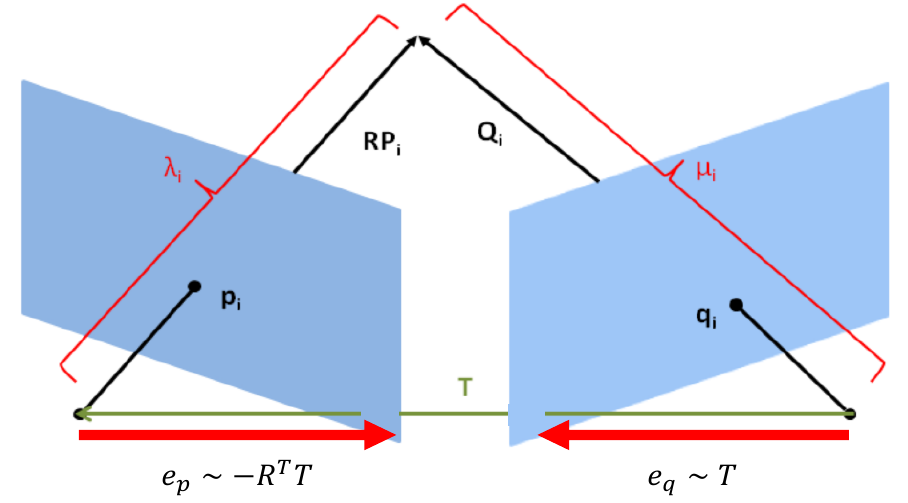
\includegraphics[width=\linewidth]{Images/SFM.png}
\begin{itemize}
  \item \textbf{Got:} 2D-2D correspondences between two views $p$, $q$.
  \item \textbf{Want:} $T, R$ between two views.
\end{itemize}
$\mu q = R \lambda p + T$\\
$T$ is here in the coordinates of $q$.\\
$DOF = 6$ (3 translation, 3 rotation), but 
we can only find the translation up to a scale. Finally, $DOF = 5$.

\subsection*{Epipolar constraint}
From the image, we see that the vectors $\mu q$, $T$ and $\lambda R p$
are coplanar. We can write the triple product:\\
$\mu q^T ( T \times \lambda R p) = 0$\\
$q^T ( T \times R p) = 0$\\
$q^T \hat{T} R p = 0$\\
$q^T E p = 0$, where $E = \hat{T} R$ essential matrix.

The planes spanned by $T$, $\lambda q$ and $\mu p$ is called epipolar
plane (cross product vanishes).

\alert{Why we cannot recover the scale?}\\
Scaling $q$ or $p$ will not violate the
constraint. Therefore, we can obtain the translation up to a scale.
\subsection*{Fundamental Matrix}
If our points are not calibrated, we have to calibrate them:\\
$F = K^{-T} \hat{T} R K'^-1$

\subsection*{Epipolar Line}
In $p$-plane, line with coefficients $E^T q$.

All epipolar lines go through the epipole $e_p$:\\
$E e_p = \hat{T} R (-R^T T) = \hat{T}T = T \times T = 0$

\subsection*{Essential Matrix Calculation}
\textbf{8-point algorithm}: because we are finding a linear solution\\
$E = \begin{pmatrix}e_1 & e_2 & e_3 \end{pmatrix}$\\
$q^T \begin{pmatrix}e_1 & e_2 & e_3 \end{pmatrix}
\begin{pmatrix}p_x \\ p_y \\ p_z \end{pmatrix}$ = 0\\
$= \begin{pmatrix}p_x q^T & p_y q^T&p_z q^T \end{pmatrix}
\begin{pmatrix}e_1 \\ e_2 \\ e_3 \end{pmatrix}$\\
$\vec{a} = \begin{pmatrix}p_x q^T & p_y q^T&p_z q^T \end{pmatrix}$
$\begin{pmatrix} a_1^T \\ a_2^T \\ \vdots \\ a_n^T \end{pmatrix} E' =
0$\\
and we do SVD. Practically: \\
$E = U \text{diag}\left(\dfrac{\sigma_1 + \sigma_2}{2}, \dfrac{\sigma_1
+ \sigma_2}{2}, 0 \right) V^T$j

\textbf{Other options for estimation}
\begin{itemize}
  \item 5 point algorithm. Quite complex. Minimum number.
  \item 7 point algorithm. Easier, don't need to do full estimation.
\end{itemize}

\alert{Always RANSAC when estimating E, we can have bad
points matches.}

\subsection*{Essential matrix properties}
$E = \hat{T} R \Rightarrow E E^T = \hat{T} \hat{T}^T$ 
$=T T^T - T^T T I$
$=\begin{pmatrix} 
  t_x^2 & t_x t_y & t_x t_z \\
  t_x t_y & t_y^2 & t_y t_z \\
  t_x t_z & t_y t_z & t_z^2
\end{pmatrix} - |T|^2 I$\\
If we solve $det(E E^T - \lambda I) = 0$, we find two eigenvalues
$|T|^2$.\\
To be essential, $E$ should have $\sigma_1 = \sigma_2 > 0$ and $\sigma_3
= 0$

\subsection*{Essential matrix decomposition}
Useful properties: \\
$\hat{Q a} = Q \hat{a} Q^T$\\
$\begin{pmatrix}
  1 & 0 & 0 \\ 0 & 1 & 0 \\ 0& 0& 0
\end{pmatrix} =\hat{T}^T_z R_{z, \pi/2}$ \\
Where\\
$T_{z, \pi/2} = \begin{pmatrix} 
  0 & 1 & 0 \\ -1 & 0 & 0\\ 0 & 0 & 0
\end{pmatrix}$

Therefore we can write
$E = \sigma U
\begin{pmatrix}
  1 & 0 & 0 \\ 0 & 1 & 0 \\ 0& 0& 0
\end{pmatrix} V^T$\\
$=\sigma \underbrace{U \hat{T}^T_z}_{\text{antisymmetric}} \quad
\underbrace{R_z V^T}_{\text{orthogonal}}$

Two $R$:
\begin{itemize}
  \item $R_1 = U R^T_{z, \pi/2} V^T$
  \item $R_2 = U R^T_{z, -\pi/2} V^T$
\end{itemize}
Two $\hat{T}$:
\begin{itemize}
  \item $T_1 = U R^T_{z, \pi/2} \Sigma U^T$
  \item $T_2 = U R^T_{z, -\pi/2} \Sigma U^T$
\end{itemize}


Finally, disambiguate with $\lambda q = \mu R p + T$ such that $\lambda,
\mu > 0$

\subsection*{Triangulation}
\begin{itemize}
  \item \textbf{Got:} $T, R$ and 2D correspondences in two images.
  \item \textbf{Want:} Depth of points in each camera $\mu_i$, $\lambda_i$.
\end{itemize}

We set the translation to $|T| = 1$
$\underbrace{\begin{pmatrix}q_i & -R p_i\end{pmatrix}}_{3\times2}
\underbrace{\begin{pmatrix} \mu_i \\\lambda_i \end{pmatrix}}_{2\times1} =
\underbrace{T}_{3 \times 1}$\\
3 eqs with 2 unknowns, solve with pseudo inverse

\subsection*{Tips and Tricks}
\begin{itemize}
  \item $R = I$, the epipolar constraint is\\
    $q^T ( T \times p) = 0$ or $(q \times p)^T T = 0$.\\
    We need 2 points to solve the problem (up to a scale).
  \item Pure translation essential matrix: we can recognize if it is
    skew symmetric. If $E$ is antisymmetric, that means that $R = I$!
\end{itemize}
